%Template da SBC para artigos em português

\documentclass[12pt]{article}

\usepackage{sbc-template}
\usepackage{graphicx,url}
\usepackage[utf8]{inputenc}
%\usepackage[brazil]{babel}
\usepackage{array}
\usepackage{tabularx}
\usepackage{booktabs}
\usepackage{amsmath}
%\usepackage[latin1]{inputenc}  

\usepackage{tikz}
\usetikzlibrary{positioning, shapes, calc}
     
\sloppy

\title{2024: Tonga's\\ Exchange Rate Policy stance }

\author{Antonio Moeaki (EFPD MOF) }


%\address{Instituto de Informática -- Universidade Federal do %Rio Grande do Sul
  %(UFRGS)\\
  %Caixa Postal 15.064 -- 91.501-970 -- Porto Alegre -- RS -- %Brazil
%\nextinstitute
  %Department of Computer Science -- University of Durham\\
 % Durham, U.K.
%\nextinstitute
%  Departamento de Sistemas e Computação\\
 % Universidade Regional de Blumenal (FURB) -- Blumenau, SC -- Brazil
%  \email{\{nedel,flavio\}@inf.ufrgs.br, R.Bordini@durham.ac.uk,
 % jomi@inf.furb.br}
%}

\begin{document} 

\maketitle

\begin{abstract}
Tonga’s economic structure is marked by a narrow production base, a reliance on imported goods, and a heavy dependence on remittances as a source of foreign exchange. Its exchange rate management is therefore crucial to its economic resilience and stability as it acts as a macroeconomic buffer stabilizing import costs and the economy's sensitivity towards external shocks. Several economic features such as Tonga's monetary policy stance, fiscal discipline, existing trade partners, history of inflation, and macroprudential policies are salient to an effective exchange rate policy. This paper attempts to capture Tonga's exchange rate policy stance and recommend strategies for future integration.



%Global events—such as financial crises, commodity price shocks, or shifts in international capital flows—can further amplify the significance of the exchange rate system a country adopts. The choice between fixed, floating, or intermediate regimes is therefore not just a technical decision, but a reflection of broader policy priorities and institutional capacities. These regimes shape how economies absorb external shocks, influence investor confidence, and affect competitiveness in international markets. In turn, they have lasting consequences for economic stability, growth prospects, and integration into the global economy.
%The purpose of the travel was to attend a seminar on ‘ST25.36 Exchange Rate Policy’, organised by the International Monetary Fund (IMF) in partnership with the Singapore Training Institute (STI). The seminar aimed to strengthen the officer’s capacity to diagnose and analyze exchange rate regimes contextualized in countries with different economic features (fiscal discipline, monetary policy stance, trade balance, history of inflation etc). The interaction of these features with the exchange rate have massive implications for the external position of the country.  
\end{abstract}


 %    \includegraphics[width=15cm]{Template_SBC/ST25.36 ERP Fun shot.jpg}


     \tableofcontents
%\begin{resumo} 
%  Este meta-artigo descreve o estilo a ser usado na confecção de artigos e
%  resumos de artigos para publicação nos anais das conferências organizadas
%  pela SBC. É solicitada a escrita de resumo e abstract apenas para os artigos
%  escritos em português. Artigos em inglês deverão apresentar apenas abstract.
 % Nos dois casos, o autor deve tomar cuidado para que o resumo (e o abstract)
  %não ultrapassem 10 linhas cada, sendo que ambos devem estar na primeira
  %página do artigo.
%\end{resumo}


\section{General Information}
\subsection{Introduction}

The National Reserve Bank of Tonga (NRBT) oversees the management of exchange rate movements  - with its mandate being to maintain (internal and external) monetary stability; to which it conducts activities in such a manner that supports macroeconomic stability and economic growth. 

\noindent For internal monetary stability, the Reserve Bank targets low and stable inflation over the medium term - a maintenance of inflation below the 5\% reference rate set by the NRBT.
For external monetary stability, an adequate amount of foreign currencies (foreign reserves) to meet the country's foreign currency demands to pay for imports and other obligations. As such, the Reserve Bank's monetary policies aim to ensure that Tonga always has foreign reserve holdings of at least three to four months of import cover.
%\subsection{Organiser Information}

%The IMF – Singapore Regional Training Institute (STI), is the International Monetary Fund’s (IMF) regional training center for the Asia and Pacific region. It provides government officials from 38 countries with training and technical assistance in macroeconomic and financial management and related legal and statistical issues. Most training takes place in two-week seminars, with shorter events organized for senior officials.


\section{Tonga's Exchange Rate Regime}
\subsection{To peg or not to peg}
Tonga's official currency is the \textit{Tongan Pa'anga}. As per the IMF, the de jure exchange rate arrangement is a \textbf{pegged exchange rate - within horizontal bands} (\textit{see Fig 1}). The external value of the pa'anga is determined on the basis of a weighted currency basket (comprising the US dollar, Australian dollar, New Zealand dollar, and Fijian dollar) - with the respective basket weights being determined by the proportions of trade with these partners.


%Diagram for exchange rates taxonomy (IMF)
\begin{figure}[h!]
\centering

%this code presets two styles we will use in this TIKz diagra,
%so we have (1) called "box" and (2) called "highlight"
% The presets in (1) make it such that its a rectangular blue box with white text
% The presets in (2) make it such that its the same but red

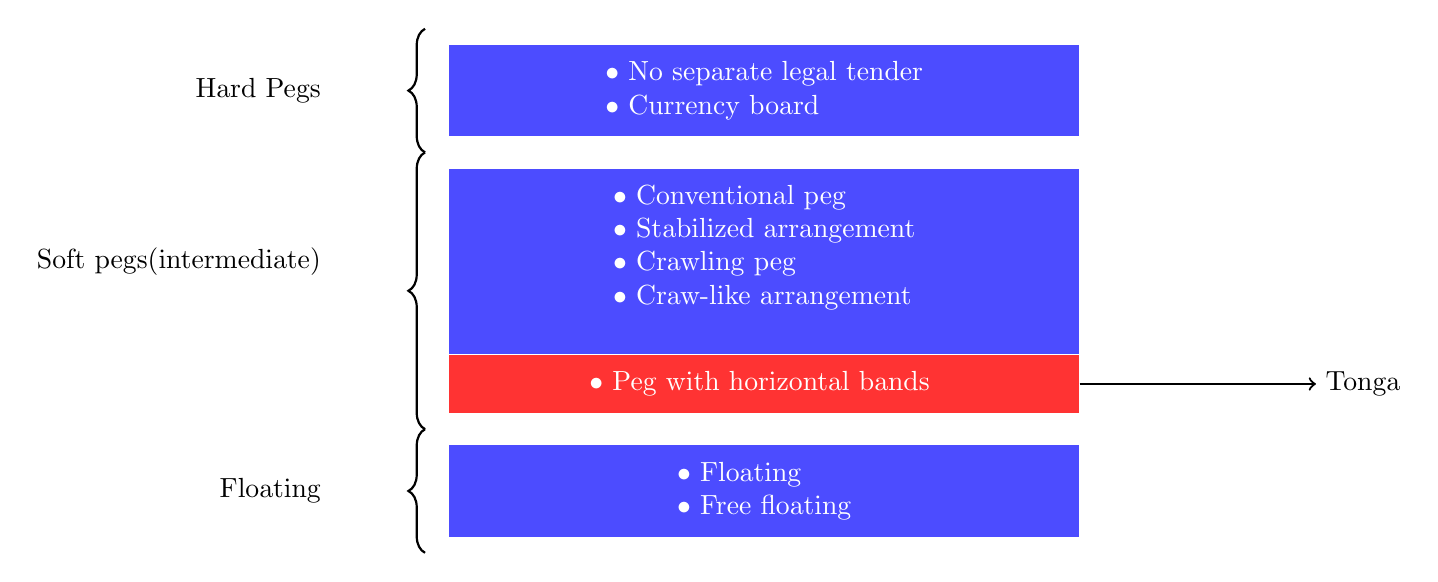
\begin{tikzpicture}[
  box/.style={
    rectangle, rounded corners=0pt, minimum width=8cm,
    text=white, font=\normalsize, align=left, fill=blue!70, inner sep=6pt
  },
  highlight/.style={
    rectangle, rounded corners=0pt, minimum width=8cm,
    text=white, font=\normalsize, align=left, fill=red!80, inner sep=6pt
  }
]

%adding NODES such as HP, SP, FLOATING
% Hard Pegs
\node[box] (hard) {
  $\bullet$ No separate legal tender \\
  $\bullet$ Currency board
};
\node[left=1.5cm of hard] (hardlabel) {Hard Pegs};

% Soft Pegs
\node[box, below=0.4cm of hard] (soft) {
  $\bullet$ Conventional peg \\
  $\bullet$ Stabilized arrangement \\
  $\bullet$ Crawling peg \\
  $\bullet$ Craw-like arrangement \\
};
\node[highlight, below=0cm of soft] (soft2) {
  $\bullet$ Peg with horizontal bands
};
\node[left=1.5cm of soft] (softlabel) {Soft pegs \\ (intermediate)};

% Floating
\node[box, below=0.4cm of soft2] (float) {
  $\bullet$ Floating \\
  $\bullet$ Free floating
};
\node[left=1.5cm of float] (floatlabel) {Floating};

% Braces
\draw[decorate,decoration={brace,amplitude=6pt,mirror},thick]
  ($(hard.north west)+(-0.3,0.2)$) -- ($(hard.south west)+(-0.3,-0.2)$);

\draw[decorate,decoration={brace,amplitude=6pt,mirror},thick]
  ($(soft.north west)+(-0.3,0.2)$) -- ($(soft2.south west)+(-0.3,-0.2)$);

\draw[decorate,decoration={brace,amplitude=6pt,mirror},thick]
  ($(float.north west)+(-0.3,0.2)$) -- ($(float.south west)+(-0.3,-0.2)$);

% Tonga node (to the right of highlighted box)
\node[right=3cm of soft2] (tonga) {Tonga};
\draw[->, thick] (soft2.east) -- (tonga.west);

\end{tikzpicture}
\caption{Exchange Rate Taxonomy}
\end{figure}

% grading scale for adv economies
%\begin{figure}[h!]
%\centering
%\begin{tikzpicture}
  % Draw scale line
%  \draw[thick] (0,0) -- (10,0);

  % Ticks
%  \foreach \x/\label in {0/Hard Peg, 5/Managed Float, 10/Floating}
%    \draw (\x,0.2) -- (\x,-0.2) node[below] {\label};

  % Gradient-style shading (optional, for "continuum")
%  \shade[left color=blue!70,right color=red!70] (0,0.4) rectangle (10,0.8);

  % Labels above scale
%  \node[above] at (0,0.8) {Stability for smaller/less developed economies};
%  \node[above] at (10,0.8) {Flexibility for larger/more advanced economies};
%\end{tikzpicture}
%\caption{Exchange rate regimes across development levels.}
%\end{figure}

\noindent The bipolar view on XR regime choice, prevalent in the late 1900s, argued that only hard pegs or free floats were viable. This was reinforced by evidence during emerging market crises (such as in Asia 1997-98, Russia 1998, Argentina 2001), which found intermediate regimes (or soft pegs) were easily vulnerable to speculative attacks and capital mobility.


\noindent However, recent studies show the evolution of exchange rate regimes has disrupted the consensus and acknowledges the choice of regime is based on a country's level of financial development, credibility and exposure to shock. For Tonga, a soft peg offers the following benefits:

\begin{itemize}
    \item  Tonga is both a net importing and remittance-dependent country. A soft peg \textbf{stabilizes the exchange rate} and acts as a buffer for other forms of economic instability. For importers, it stabilizes the cost of essential goods. For families, it stabilizes the value of remittances sent home.

    \item Tonga has a very small and underdeveloped financial system. According to the AREAER (2024), there are no deep foreign exchange markets or sophisticated hedging instruments (like futures or options) that businesses could use to protect themselves against currency fluctuations. 
\end{itemize}

%\newpage


%\section{Transition to Flexible ER}

%lol i need some text here 


\section{External Balance Assessment}
\subsection{EBA-Lite model}


\begin{table}[h!]
\centering
\renewcommand{\arraystretch}{1.3} % row spacing

\begin{tabular}{@{}l r@{}} % normal tabular, no extra stretch
\hline
 & \textbf{CA model} \\
\hline
\textbf{CA-Actual} & \textbf{-7.1} \\
\quad Cyclical Contributions (from model) (-) & -0.1 \\
\quad Additional temporary/Statistical factors (-) 1/ & 0.0 \\
\quad Natural disasters and conflicts & 0.7 \\
\textbf{Adjusted CA} & \textbf{-8.0} \\[6pt]

\textbf{CA Norm (from model) 2/} & \textbf{-8.0} \\
\quad Adjustment to the norm & 0.0 \\
\textbf{Adjusted CA Norm} & \textbf{-8.0} \\[6pt]

\textbf{CA Gap} & \textbf{0.0} \\
\quad o/w Policy gap & 4.2 \\[6pt]

Elasticity & -0.3 \\
\textbf{REER Gap (in percent)} & \textbf{-0.1} \\
\hline
\end{tabular}

\vspace{2pt}

% Align source with start of table:
\centering
\quad \quad \parbox{\linewidth}{\hspace{0pt}\footnotesize Source: IMF staff estimates.}

\end{table}
The EBA-lite CA model estimates the adjusted CA balance at -8.0 percent of GDP and the 
adjusted CA norm at -8.0 percent of GDP. With a gap close to 0 percent of GDP, the external position in 
FY2024 is assessed to be broadly in line with medium-term fundamentals and desirable policies (text table). 
The policy gap (4.2 percent of GDP) primarily reflects the relatively looser fiscal policy in the rest of the 
world


\section{Early Warning System for Crises}
\subsection{Constructing the Exchange Market Pressure index}

Financial crises (currency, banking, or debt) are costly. The Early Warning System acts as a surveillance tool to identify vulnerabilities (in country fundamentals) and triggers (econonmic shocks) that could lead to crises episodes. This system utilizes regression analysis to predict crises, but first requires the construction of a binary dependent variable that signals (1) for a crisis and (0) otherwise.

\noindent \: \: The \textbf{Exchange Market Pressure (EMP)} index will be used for this dependent variable construction:

$$EMP = \frac{\Delta e}{e} - \frac{\sigma_{e}}{\sigma_{fx}} \left(\frac{\Delta fxr}{fxr}\right),$$

\noindent which notes $\frac{\Delta e}{e}$ as the percentage change in nominal exchange rate (e) , $\left(\frac{\Delta fxr}{fxr}\right)$ as the percentage change in foreign exchange reserves (fxr), with $\sigma_{e}$ and $\sigma_{fxr}$ as the respective volatility of (e) and (fxr). 

\noindent This EMP index is converted to a crisis indicator (c) - equal to 1 for a crisis, and 0 for a tranquil period - considering the movements of the EMP index with respect to the historical mean and standard deviation. Mathematically, this is represented as:

  \begin{equation*}
   %     \text{Is \(b_{i+1}\leqslant b_i\) \& \(\lim_{i\to\infty}b_i=0\)?}\:
   c \rightarrow
        \begin{cases}
            \text{1}, & EMP > \mu_{EMP} + \varphi \sigma_{EMP} \\
            \text{0},  & EMP \leq \mu_{EMP} + \varphi \sigma_{EMP}
        \end{cases}
    \end{equation*}

where $\mu_{EMP}$ is the sample mean and $\sigma_{EMP}$ is the sample standard deviation. The $\varphi$ is chosen arbritrarily ( $1.5<\varphi <3$ ), keeping in mind not to set it too high (as to incur type 2 errors and miss crisis episodes) or to set it too low (and to incur type 1 errors and issue false alarms). 

\subsection{Historical financial Crises}
For Tonga, data from January 2012 to May 2025 has been collected for both nominal exchange rates (e) (in USD) and foreign reserves (fxr), which yielded the following calculations:


    \begin{table}[h]
        \centering
        \begin{tabular}{llllll}
          \toprule
            \sigma_{e}  &  \sigma_{fxr}  &  \mu_{emp}  & \mu_{emp}  & \varphi \\
            \midrule
            1.05  &  3.16   &   -0.43   &  1.12   & 1.85 \\
            \bottomrule
        \end{tabular}
    \end{table}

    
	\begin{figure}[h]
    		\centering
    		\includegraphics[width=0.9\columnwidth]{Template_SBC/template-latex/EMP.png}
    		%\caption{}
    		\label{fig:RSE}
    \end{figure}


    


The historical data marks \textbf{February 2016} and \textbf{September 2022} as two periods where Tonga's nominal exchange rates (e) and foreign reserves (fxr) fluctated abnormally as to indicate a crisis. For february 2016, i gather there was a large-scale non-performing loan cancellation from the bank for the agricultural sector  due to the failure in exports for the squash sector.

For September 2022, 

\section{Foreign Reserve Adequacy}
Tonga’s official foreign reserves are slowly 
declining but still remained well above 
minimum adequacy thresholds providing 
continued support for external stability.
Foreign reserves declined in the year to 
February 2025 by 2.9 percent ($26.0 m) to 
$865.4m. The annual decline in foreign 
reserves corresponds to the higher outflows 
for import payments, offshore investments, 
and repayments of external debt. The 
current level of foreign reserves is 
equivalent to 9.9 months of imports 
coverage, lower than the 11.5 months of 
A-Figure 15: Remittance by Currency.
Source: NRBT OET.
A-Figure 16: Gross Official Foreign Reserves.
Source: NRBT; Tonga Statistics Department.
Government of Tonga Budget Statement for the year ending 30th June 2026
89
imports coverage in February 2024. Nonetheless, the current level of foreign reserves is still above the 
IMF prescribed level of 7.5 months of imports cover, and the NRBT’s minimum threshold of 3 months 
of imports cover. 
The announcement of AUD\$85m and other donor funds to be received in the next few years would also 
help maintain the level of foreign reserves. However, the anticipated increase in import payments 
relative to the anticipated gradual slowdown in foreign aid and remittances are expected to gradually 
reduce the level of foreign reserves. Foreign reserves are mostly held in USD, AUD, and NZD. The 
outlook for foreign reserves is expected to remain comfortable in the near to medium-term and ongoing 
monitoring is essential to ensure the foreign reserves remain sufficient amid external pressures
\subsection{months of imports}
\subsection{Short term debt}
\subsection{third way lol}
\section{Tonga Under Covid Conditions}
\section{Workshops}

\textbf{Workshop 1: Choice of exchange rate regime} \\

     Group 1 presented on a hypothetical country (Country Durian) which exhibits the following features: Strong fiscal discipline with a GDP growth of 1-3\% consistently, a diversifiable export base, \\
\textbf{Workshop 2: Transition from fixed to flexible exchange rate regime} \\
\textbf{Workshop 3: External Balance Assessment} \\



\begin{table}[h!]
\centering
\renewcommand{\arraystretch}{1.3} % row spacing

\begin{tabular}{@{}l r@{}} % normal tabular, no extra stretch
\hline
 & \textbf{CA model} \\
\hline
\textbf{CA-Actual} & \textbf{-7.1} \\
\quad Cyclical Contributions (from model) (-) & -0.1 \\
\quad Additional temporary/Statistical factors (-) 1/ & 0.0 \\
\quad Natural disasters and conflicts & 0.7 \\
\textbf{Adjusted CA} & \textbf{-8.0} \\[6pt]

\textbf{CA Norm (from model) 2/} & \textbf{-8.0} \\
\quad Adjustment to the norm & 0.0 \\
\textbf{Adjusted CA Norm} & \textbf{-8.0} \\[6pt]

\textbf{CA Gap} & \textbf{0.0} \\
\quad o/w Policy gap & 4.2 \\[6pt]

Elasticity & -0.3 \\
\textbf{REER Gap (in percent)} & \textbf{-0.1} \\
\hline
\end{tabular}

\vspace{2pt}

% Align source with start of table:
\centering
\quad \quad \parbox{\linewidth}{\hspace{0pt}\footnotesize Source: IMF staff estimates.}

\end{table}
The EBA-lite CA model estimates the adjusted CA balance at -8.0 percent of GDP and the 
adjusted CA norm at -8.0 percent of GDP. With a gap close to 0 percent of GDP, the external position in 
FY2024 is assessed to be broadly in line with medium-term fundamentals and desirable policies (text table). 
The policy gap (4.2 percent of GDP) primarily reflects the relatively looser fiscal policy in the rest of the 
world



       Doing an EBA analysis of country Poland, we evaluate their REER gap is -7.3\% which was in alignment with IMF’s article IV EBA results for 2024. This implied their currency was undervalued and needed to appreciate by 7.3\% in real terms to close the CA\_gap of 1.5\% - which came from the cyclical components of trade\_openness \\
\textbf{Workshop 4: Early Warning Crises} \\

\textbf{Workshop 5: Foreign Exchange Reserve Adequacy} \\
\textbf{Workshop 6: Covid-19 Case study}	


\subsection{ST25.36 Exchange Rate Policy}

For ST25.36, the course focused on key exchange rate rate concepts (real, nominal, bilateral, multilateral, spot, forward) and arbitrage conditions (UIP, law of one price, PPP, relative PPP); its role in achieving internal and external balance (adjustment to overall equilibrium under floating and fixed exchange rate regimes); its role in economic growth (undervaluation, Washington Consensus, the Balassa-Samuelson effect).

Exchange rate policy and regimes (taxonomy, impossible trinity) and associated policy mix (monetary policy independence, financial stability, fiscal policy, capital controls).  

Practical Problems of Exchange Rate Policy in Developing and Emerging Market Economies (concerns of excessive volatility; de jure vs. de facto regimes; competitiveness, price stability; exchange-rate pass-through; targets and instruments).  

Transitions from rigid to flexible exchange rates regimes (motives; speed of transition; deep and liquid domestic FX markets, derivatives markets, coherent intervention policy, nominal anchor; transition sequence).   
FX interventions (sterilized or non-sterilized; motivations, channels, effectiveness, instruments, tactics, policy communication).  

The learnings of this paper will be applied in the context of \textbf{Tonga}.



%\section{Sections and Paragraphs}

%Section titles must be in boldface, 13pt, flush left. There should be an extra
12 pt of space before each title. Section numbering is optional. The first
paragraph of each section should not be indented, while the first lines of
subsequent paragraphs should be indented by 1.27 cm.

%\subsection{Subsections}

%The subsection titles must be in boldface, 12pt, flush left.

%\section{Figures and Captions}\label{sec:figs}


%Figure and table captions should be centered if less than one line
%(Figure~\ref{fig:exampleFig1}), otherwise justified and indented by 0.8cm on
%both margins, as shown in Figure~\ref{fig:exampleFig2}. The caption font must
%be Helvetica, 10 point, boldface, with 6 points of space before and after each
%caption.

%\begin{figure}[ht]
%\centering
%\includegraphics[width=.5\textwidth]{fig1.jpg}
%caption{A typical figure}
%\label{fig:exampleFig1}
%\end{figure}

%\begin{figure}[ht]
%\centering
%\includegraphics[width=.3\textwidth]{fig2.jpg}
%\caption{This figure is an example of a figure caption taking more than one
%  line and justified considering margins mentioned in Section~\ref{sec:figs}.}
%\label{fig:exampleFig2}
%\end{figure}

%In tables, try to avoid the use of colored or shaded backgrounds, and avoid
%thick, doubled, or unnecessary framing lines. When reporting empirical data,
%do not use more decimal digits than warranted by their precision and
%reproducibility. Table caption must be placed before the table (see Table 1)
%nd the font used must also be Helvetica, 10 point, boldface, with 6 points of
%space before and after each caption.

%\begin{table}[ht]
%\centering
%\caption{Variables to be considered on the evaluation of interaction
%  techniques}
%\label{tab:exTable1}
%\includegraphics[width=.7\textwidth]{table.jpg}
%\end{table}

%\section{Images}

%All images and illustrations should be in black-and-white, or gray tones,
%excepting for the papers that will be electronically available (on CD-ROMs,
%internet, etc.). The image resolution on paper should be about 600 dpi for
%black-and-white images, and 150-300 dpi for grayscale images.  Do not include
%images with excessive resolution, as they may take hours to print, without any
%visible difference in the result. 

%\section{References}

%Bibliographic references must be unambiguous and uniform.  We recommend giving
%the author names references in brackets, e.g. \cite{knuth:84},
%\cite{boulic:91}, and \cite{smith:99}.

%The references must be listed using 12 point font size, with 6 points of space
%before each reference. The first line of each reference should not be
%indented, while the subsequent should be indented by 0.5 cm.

\bibliographystyle{sbc}
\bibliography{sbc-template}

\end{document}
